\chapter{Multi-Agent Software Systems}
\label{chap:multi-agent-siakad}

\section*{Tujuan Pembelajaran}
\begin{enumerate}
  \item Menjelaskan arsitektur sistem multi-agen (MAS) berbasis Model Context Protocol (MCP) untuk orkestrasi tugas otomatis pada sistem web perusahaan.
  \item Menerapkan pola \textit{Orchestrator-Worker} dalam pendistribusian tugas dari pemrosesan data jadwal (CSV/Excel) ke otomasi browser (Playwright), termasuk merancang \textit{task queue} berbasis berkas JSON sebagai mekanisme komunikasi antar-agen.
  \item Mengimplementasikan server MCP modular untuk pembaca data jadwal, otomasi browser, dan \textit{shared state}, sekaligus menganalisis \textit{trade-off} pendekatan agen tunggal dan multi-agen dari sisi skalabilitas, keandalan, efisiensi konteks, dan penalaran visual.
\end{enumerate}

\section{Pendahuluan}

Pengisian Berita Acara Perkuliahan (BAP) dan daftar hadir pada sistem informasi akademik seperti SIAKAD merupakan tugas administratif yang repetitif bagi tenaga pengajar. Setiap sesi perkuliahan memerlukan langkah-langkah yang identik: autentikasi ke portal, navigasi ke halaman daftar hadir, pemilihan semester dan tanggal, identifikasi baris kelas yang tepat pada tabel jadwal, serta pengisian topik dan deskripsi pembahasan melalui formulir \textit{popup}. Meskipun terlihat sederhana, proses ini rentan terhadap kesalahan manusia (\textit{human error}) dan memakan waktu yang signifikan jika dilakukan secara manual untuk banyak mata kuliah dan banyak sesi.

Otomasi tradisional menggunakan skrip statis (misalnya Selenium script) sering kali gagal menghadapi perubahan antarmuka web yang dinamis, elemen \textit{date picker} yang menggunakan JavaScript kustom, atau prosedur autentikasi yang kompleks. Di sisi lain, penggunaan agen kecerdasan buatan (AI) tunggal berbasis Large Language Model (LLM) sering kali terbentur pada keterbatasan jendela konteks (\textit{context window}) --- memuat seluruh data jadwal dan riwayat interaksi browser dalam satu agen menghabiskan kuota token dengan cepat dan menurunkan akurasi instruksi.

Bab ini membahas implementasi sistem otomasi pengisian kehadiran SIAKAD menggunakan pendekatan \textbf{Multi-Agent System (MAS)} yang diorkestrasi melalui \textbf{Model Context Protocol (MCP)}. Dengan memisahkan tanggung jawab antara \textbf{Claude} sebagai \textit{Orchestrator} (perencana dan pengirim tugas) dan \textbf{Gemini} sebagai \textit{Browser Worker} (pelaksana otomasi browser), sistem ini mampu menangani alur kerja yang kompleks secara lebih andal dan efisien. Komunikasi antar-agen dilakukan melalui \textit{shared task queue} berbasis berkas JSON yang dikelola oleh server MCP \texttt{shared-state}.

\section{Deskripsi Masalah Domain yang Diselesaikan}

\subsection{Konteks Domain}

Domain yang dibahas adalah otomasi administrasi akademik pada SIAKAD Universitas Pradita (\texttt{siakad.pradita.ac.id}). Fokus utamanya adalah pengisian formulir Berita Acara Perkuliahan yang melibatkan input teks (\textit{Topik} dan \textit{Deskripsi Pembahasan}) berdasarkan data jadwal yang tersimpan dalam format CSV atau Excel.

Sistem harus mampu melakukan:
\begin{enumerate}
  \item Membaca data jadwal dari berkas sumber di direktori \texttt{schedule-data/}, satu berkas per mata kuliah.
  \item Mengelola antrean tugas (\textit{task queue}) yang persisten untuk memastikan setiap sesi terisi tepat satu kali dan mendukung \textit{retry} jika terjadi kegagalan.
  \item Berinteraksi dengan elemen web yang memiliki \textit{ID} atau \textit{class name} yang dinamis, termasuk \textit{date picker}, \textit{dropdown} semester, dan tabel jadwal.
  \item Melakukan validasi pasca-pengisian menggunakan tangkapan layar (\textit{screenshot}) dan pengecekan pesan notifikasi sukses.
\end{enumerate}

\begin{figure}[htbp]
\centering
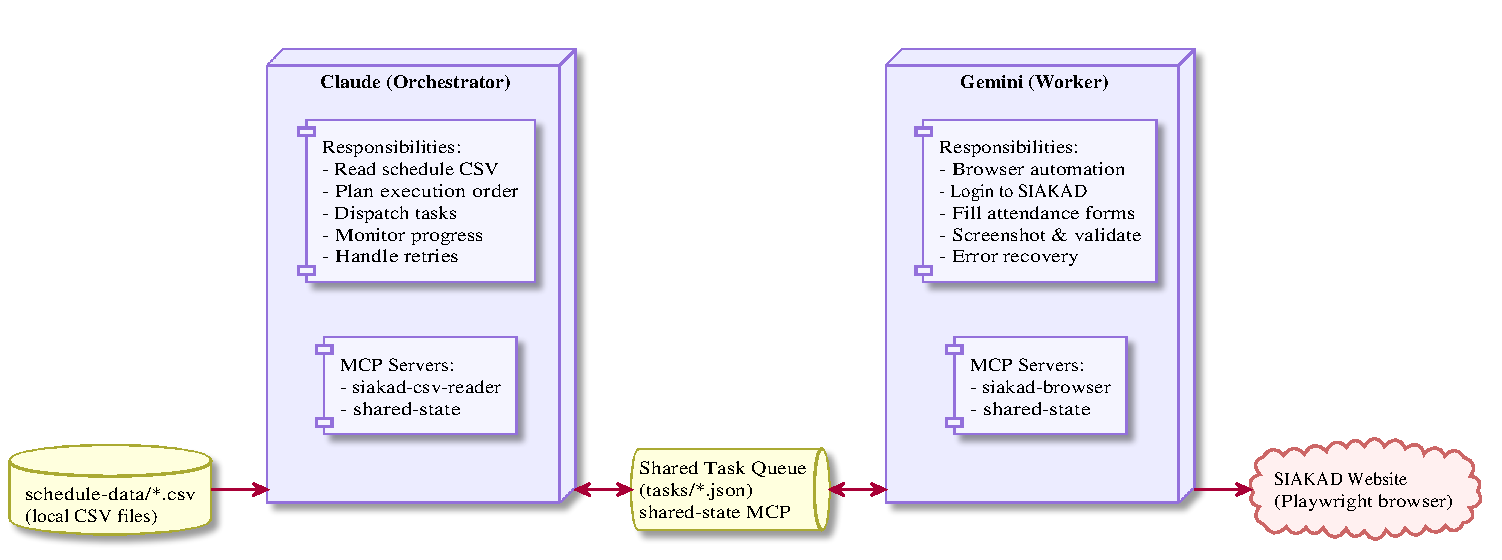
\includegraphics[width=\textwidth]{../figures/architecture.pdf}
\caption{Arsitektur Multi-Agent SIAKAD: Claude sebagai Orchestrator membaca data CSV dan mendistribusikan tugas melalui Shared Task Queue, sementara Gemini sebagai Browser Worker mengeksekusi otomasi browser ke portal SIAKAD.}
\label{fig:ch14-architecture}
\end{figure}

Gambar~\ref{fig:ch14-architecture} menunjukkan arsitektur keseluruhan sistem. Terdapat empat komponen utama: data jadwal CSV sebagai input, Claude (Orchestrator) yang membaca dan merencanakan eksekusi, Shared Task Queue sebagai jembatan komunikasi, dan Gemini (Worker) yang mengeksekusi otomasi browser terhadap portal SIAKAD.

\subsection{Target Model Otomasi}

Target dari sistem ini adalah keberhasilan pengisian Berita Acara Perkuliahan pada portal SIAKAD untuk seluruh baris jadwal yang terdapat dalam berkas CSV. Proses ini direpresentasikan dalam urutan tugas yang dikelola secara persisten dalam format JSON di direktori \texttt{tasks/}.

\begin{lstlisting}[
  language=json,
  caption={Representasi tugas dalam format JSON dengan status \texttt{pending}},
  label={lst:ch14-task-json},
  basicstyle=\ttfamily\scriptsize
]
{
  "id": "task_002",
  "type": "fill_attendance",
  "status": "pending",
  "params": {
    "tanggal": "2026-01-21",
    "mata_kuliah": "Advanced Software Engineering & DevOps",
    "kelompok_kelas": null,
    "semester": "2025/2026 GENAP",
    "topik": "Session-001: General Lecture",
    "deskripsi": "Overview of course objectives, evaluation methods,
                  and introduction to modern software engineering
                  and DevOps practices"
  },
  "result": null,
  "error": null,
  "created_at": "2026-04-04 10:30:15",
  "updated_at": null
}
\end{lstlisting}

\noindent Listing~\ref{lst:ch14-task-json} memperlihatkan struktur lengkap sebuah tugas. Setiap tugas memiliki \texttt{id} unik, \texttt{type} yang menentukan jenis operasi (\texttt{login}, \texttt{fill\_attendance}, \texttt{close\_browser}), \texttt{status} yang melacak progres (\texttt{pending} $\rightarrow$ \texttt{in\_progress} $\rightarrow$ \texttt{completed}/\texttt{failed}), serta \texttt{params} yang berisi parameter input. Pemisahan data tugas dari logika agen memungkinkan sistem untuk melakukan \textit{retry} jika terjadi kegagalan tanpa kehilangan status pengerjaan secara keseluruhan.

\subsection{Masalah Utama}

Permasalahan yang mendorong penggunaan sistem multi-agen pada domain ini adalah:
\begin{enumerate}
  \item \textbf{Kompleksitas Navigasi Web.} SIAKAD memiliki alur navigasi yang melibatkan \textit{dropdown} semester, \textit{date picker} dengan format tanggal yang bervariasi (YYYY-MM-DD vs DD/MM/YYYY vs MM/DD/YYYY), tabel jadwal dengan jumlah baris dinamis yang berubah setiap tanggal, dan formulir \textit{popup/modal} yang memerlukan penanganan khusus.
  \item \textbf{Keterbatasan Context Window.} Memberikan seluruh kode sumber otomasi, data jadwal lengkap (15+ sesi $\times$ beberapa mata kuliah), dan riwayat interaksi browser ke satu agen LLM menyebabkan degradasi akurasi instruksi secara signifikan.
  \item \textbf{Kebutuhan akan Spesialisasi.} Perencanaan jadwal memerlukan ketelitian dalam pemrosesan teks dan logika sekuensial (kekuatan Claude), sedangkan interaksi browser memerlukan pemahaman visual terhadap elemen halaman web dan eksekusi alat yang presisi (kekuatan Gemini dengan kemampuan \textit{visual reasoning}).
  \item \textbf{Ketahanan terhadap Error.} Jika satu sesi browser gagal (misalnya \textit{timeout} pada \textit{date picker}), sistem harus mampu melanjutkan ke tugas berikutnya atau mencoba kembali tugas yang gagal tanpa mengulang seluruh proses perencanaan dari awal.
\end{enumerate}

\subsection{Kebutuhan Pemodelan Sistem}

Berdasarkan masalah di atas, kebutuhan sistem untuk otomasi SIAKAD adalah:
\begin{enumerate}
  \item \textbf{Protokol Komunikasi Standar (MCP).} Model Context Protocol diperlukan untuk menghubungkan agen LLM dengan alat bantu (\textit{tools}) secara terstandar, sehingga setiap server MCP dapat digunakan oleh berbagai model LLM tanpa modifikasi.
  \item \textbf{Shared State Mechanism} melalui \textit{task queue} berbasis berkas JSON di direktori \texttt{tasks/} sebagai mekanisme sinkronisasi antar-agen yang sederhana, persisten, dan mudah di-debug.
  \item \textbf{Orchestrator Agent} yang bertugas membaca seluruh jadwal dari CSV, memvalidasi kelengkapan data, membuat antrean tugas secara sekuensial, dan memantau penyelesaian setiap tugas.
  \item \textbf{Worker Agent} yang fokus pada eksekusi perintah browser melalui Playwright, penanganan formulir \textit{modal}, validasi keberhasilan melalui \textit{screenshot} dan pengecekan pesan notifikasi, serta pelaporan hasil kembali ke \textit{task queue}.
\end{enumerate}

Kebutuhan ini menjadi dasar perancangan arsitektur tiga server MCP (\texttt{siakad-csv-reader}, \texttt{siakad-browser}, dan \texttt{shared-state}) yang dibahas pada bagian implementasi.

\section{Metodologi Multi-Agen berbasis MCP}

Sistem ini menggunakan Model Context Protocol (MCP) sebagai lapisan abstraksi antara agen kecerdasan buatan dan \textit{host resources}. MCP menyediakan mekanisme standar bagi LLM untuk memanggil \textit{tools} eksternal melalui transport \texttt{stdio}, sehingga server MCP dapat digunakan oleh berbagai model tanpa modifikasi. Metodologi pengembangannya mengikuti tujuh langkah berikut.

\subsection{Langkah 1: Analisis Domain dan Identifikasi Peran Agen}

Langkah pertama adalah menganalisis domain otomasi dan mengidentifikasi peran yang diperlukan. Pada domain ini, dua peran utama diidentifikasi:
\begin{itemize}
  \item \textbf{Orchestrator (Perencana):} Bertanggung jawab atas pembacaan data jadwal, validasi kelengkapan, serta pembuatan dan pemantauan antrean tugas. Peran ini memerlukan ketelitian dalam pemrosesan teks dan logika sekuensial.
  \item \textbf{Worker (Pelaksana):} Bertanggung jawab atas eksekusi otomasi browser, termasuk login, navigasi halaman, pengisian formulir, dan validasi visual. Peran ini memerlukan kemampuan penalaran visual.
\end{itemize}

\textbf{Input tahap ini:} Deskripsi proses bisnis manual yang akan diotomasi.

\textbf{Output tahap ini:} Daftar peran agen beserta tanggung jawab masing-masing dan model LLM yang paling sesuai.

\subsection{Langkah 2: Perancangan Protokol Komunikasi (MCP)}

MCP dipilih sebagai protokol komunikasi karena menyediakan:
\begin{itemize}
  \item \textbf{Transport standar (\texttt{stdio}):} Server MCP dapat dijalankan sebagai proses terpisah dan berkomunikasi dengan agen melalui \textit{standard input/output}.
  \item \textbf{Tool discovery otomatis:} Agen LLM secara otomatis menemukan daftar \textit{tools} yang tersedia pada setiap server MCP.
  \item \textbf{Dekopling agen-tool:} Server MCP tidak bergantung pada model LLM tertentu --- server yang sama dapat digunakan oleh Claude CLI maupun Gemini CLI.
\end{itemize}

\textbf{Input tahap ini:} Daftar peran agen dan kemampuan yang dibutuhkan.

\textbf{Output tahap ini:} Daftar server MCP yang diperlukan beserta pembagian tool per server.

\subsection{Langkah 3: Definisi Antarmuka Tool per Server MCP}

Setiap server MCP mendefinisikan sekumpulan \textit{tools} yang dapat dipanggil oleh agen. Definisi tool meliputi nama, deskripsi, parameter (dengan tipe dan nilai default), serta format kembalian. Pada proyek ini, tiga server MCP dirancang:
\begin{enumerate}
  \item \textbf{\texttt{siakad-csv-reader}} (4 tools): membaca dan memfilter data jadwal dari CSV/Excel.
  \item \textbf{\texttt{siakad-browser}} (15 tools): otomasi browser melalui Playwright untuk interaksi dengan SIAKAD.
  \item \textbf{\texttt{shared-state}} (6 tools): manajemen antrean tugas berbasis berkas JSON.
\end{enumerate}

\textbf{Input tahap ini:} Daftar server MCP dan skenario penggunaan.

\textbf{Output tahap ini:} Spesifikasi API setiap tool (nama, parameter, deskripsi, contoh kembalian).

\subsection{Langkah 4: Perancangan Task Queue dan State Machine}

Task queue dirancang sebagai kumpulan berkas JSON di direktori \texttt{tasks/}. Setiap berkas merepresentasikan satu tugas dengan \textit{state machine} sebagai berikut:

\begin{center}
\texttt{pending} $\xrightarrow{\text{Worker claims}}$ \texttt{in\_progress} $\xrightarrow{\text{success}}$ \texttt{completed}
\end{center}
\begin{center}
\texttt{in\_progress} $\xrightarrow{\text{failure}}$ \texttt{failed}
\end{center}

Desain ini memiliki keunggulan: berkas JSON dapat di-\textit{inspect} secara manual, persisten terhadap restart proses, dan tidak memerlukan database eksternal.

\textbf{Input tahap ini:} Jenis tugas dan transisi status yang diizinkan.

\textbf{Output tahap ini:} Skema JSON tugas dan aturan transisi status.

\subsection{Langkah 5: Penyusunan Agent Prompt Engineering}

Setiap agen memerlukan instruksi (\textit{prompt}) yang mendefinisikan perannya, daftar tool yang tersedia, alur kerja yang harus diikuti, dan aturan penanganan kesalahan. Prompt disimpan sebagai berkas Markdown di direktori \texttt{agents/}:
\begin{itemize}
  \item \texttt{orchestrator\_prompt.md} --- instruksi untuk Claude sebagai Orchestrator.
  \item \texttt{worker\_prompt.md} --- instruksi untuk Gemini sebagai Browser Worker.
\end{itemize}

\textbf{Input tahap ini:} Spesifikasi tool dan alur kerja target.

\textbf{Output tahap ini:} Berkas prompt Markdown untuk setiap agen.

\subsection{Langkah 6: Implementasi dan Integrasi}

Implementasi meliputi penulisan kode server MCP (Python), konfigurasi skrip peluncuran (\texttt{run.sh}), dan integrasi seluruh komponen melalui skrip master (\texttt{run\_multiagents.sh}). Integrasi memastikan:
\begin{itemize}
  \item Server MCP terdaftar pada kedua CLI agen (Claude dan Gemini).
  \item Kredensial dan URL dimuat dari \texttt{config.json} yang terpusat.
  \item Gemini diluncurkan terlebih dahulu (sebagai Worker yang melakukan \textit{polling}), diikuti Claude (sebagai Orchestrator yang mendistribusikan tugas).
\end{itemize}

\textbf{Input tahap ini:} Spesifikasi tool, prompt, dan konfigurasi.

\textbf{Output tahap ini:} Sistem multi-agen yang berfungsi end-to-end.

\subsection{Langkah 7: Pengujian End-to-End}

Pengujian dilakukan dengan menjalankan sistem terhadap data jadwal nyata dan memverifikasi bahwa setiap sesi terisi dengan benar pada portal SIAKAD. Bukti keberhasilan berupa \textit{screenshot} per sesi dan laporan ringkasan dari Orchestrator.

\textbf{Input tahap ini:} Berkas CSV jadwal dan akses ke portal SIAKAD.

\textbf{Output tahap ini:} Laporan keberhasilan dan \textit{screenshot} bukti pengisian.
\section{Implementasi Detail}

Bagian ini membahas implementasi lengkap sistem multi-agen SIAKAD, mulai dari arsitektur proyek, konfigurasi, hingga kode sumber setiap server MCP dan skrip peluncuran.

\subsection{Arsitektur Implementasi}

Proyek ini disusun dalam struktur modular yang memisahkan logika server MCP dari instruksi agen (\textit{prompts}) dan data jadwal.

\begin{lstlisting}[
  language=bash,
  caption={Struktur direktori proyek Multi-Agent SIAKAD},
  label={lst:ch14-project-structure},
  basicstyle=\ttfamily\scriptsize
]
session-14/
|-- README.md                         # Dokumentasi proyek
|-- CLAUDE.md                         # Instruksi konteks untuk Claude CLI
|-- GEMINI.md                         # Instruksi konteks untuk Gemini CLI
|-- config.json                       # Kredensial dan URL SIAKAD
|-- schedule-data/                    # Data jadwal CSV (satu per mata kuliah)
|   +-- advanced_software_engineering_and_devops.csv
|-- mcp-servers/                      # Server MCP (tool layer)
|   |-- browser-automation/
|   |   |-- server.py                 # Playwright browser automation (15 tools)
|   |   +-- run.sh                    # Skrip peluncur
|   +-- csv-reader/
|       |-- server.py                 # Pembaca CSV/Excel (4 tools)
|       +-- run.sh                    # Skrip peluncur
|-- agents/                           # Komponen multi-agen
|   |-- shared_state.py               # Task queue MCP server (6 tools)
|   |-- run_shared_state.sh           # Skrip peluncur
|   |-- orchestrator_prompt.md        # Instruksi Claude (Orchestrator)
|   +-- worker_prompt.md              # Instruksi Gemini (Worker)
|-- tasks/                            # Berkas tugas JSON (dibuat saat runtime)
|-- run_multiagents.sh                # Mode multi-agen (Claude + Gemini)
|-- run_claude_only.sh                # Mode agen tunggal (Claude saja)
|-- run_claude_interactive.sh         # Mode interaktif (Claude)
+-- run_gemini_only.sh                # Mode agen tunggal (Gemini saja)
\end{lstlisting}

\noindent Listing~\ref{lst:ch14-project-structure} memperlihatkan pemisahan yang jelas antara tiga lapisan: \textit{data layer} (\texttt{schedule-data/} dan \texttt{config.json}), \textit{tool layer} (\texttt{mcp-servers/} dan \texttt{agents/shared\_state.py}), dan \textit{agent layer} (\texttt{agents/*.md} dan skrip peluncuran). Pemisahan ini memungkinkan modifikasi independen pada setiap lapisan tanpa memengaruhi lapisan lain.

\subsection{Konfigurasi Sistem}

Seluruh kredensial dan URL dikonfigurasi dalam satu berkas \texttt{config.json} yang dimuat oleh setiap server MCP saat startup.

\begin{lstlisting}[
  language=json,
  caption={Konfigurasi SIAKAD pada config.json},
  label={lst:ch14-config-json},
  basicstyle=\ttfamily\scriptsize
]
{
  "siakad": {
    "login_url": "https://siakad.pradita.ac.id/login",
    "daftar_hadir_url": "https://siakad.pradita.ac.id/dosen/daftar_hadir",
    "username": "dosen@pradita.ac.id",
    "password": "********"
  },
  "schedule_dir": "./schedule-data"
}
\end{lstlisting}

Data jadwal disimpan dalam format CSV dengan kolom-kolom berikut:

\begin{table}[h]
\centering
\caption{Format kolom CSV data jadwal}
\label{tab:ch14-csv-format}
\footnotesize
\begin{tabular}{|>{\raggedright\arraybackslash}p{0.17\textwidth}|>{\centering\arraybackslash}p{0.09\textwidth}|>{\raggedright\arraybackslash}p{0.55\textwidth}|}
\hline
\textbf{Kolom} & \textbf{Wajib} & \textbf{Deskripsi} \\
\hline
\texttt{no} & Tidak & Nomor sesi perkuliahan (untuk referensi) \\
\hline
\texttt{semester} & Tidak & Nama semester, misalnya \texttt{2025/2026 GENAP} \\
\hline
\texttt{tanggal} & Ya & Tanggal dalam format \texttt{YYYY-MM-DD} \\
\hline
\texttt{mata\_kuliah} & Ya & Nama mata kuliah (harus cocok dengan tampilan SIAKAD) \\
\hline
\texttt{kelompok\_kelas} & Tidak & Kelompok kelas, misalnya \texttt{Kelas A}; \texttt{-} jika tidak ada \\
\hline
\texttt{topik} & Ya & Topik perkuliahan yang akan diisi ke formulir \\
\hline
\texttt{deskripsi} & Ya & Deskripsi pembahasan yang akan diisi ke formulir \\
\hline
\end{tabular}
\normalsize
\end{table}

\begin{lstlisting}[
  language=bash,
  caption={Contoh data jadwal dalam format CSV},
  label={lst:ch14-csv-sample},
  basicstyle=\ttfamily\scriptsize
]
no,semester,tanggal,mata_kuliah,kelompok_kelas,topik,deskripsi
1,2025/2026 GENAP,2026-01-21,Advanced Software Engineering & DevOps,-,
  Session-001: General Lecture,"Overview of course objectives,
  evaluation methods, and introduction to modern software
  engineering and DevOps practices"
2,2025/2026 GENAP,2026-01-28,Advanced Software Engineering & DevOps,-,
  Session-002: Docker-based Software System,"Building and
  demonstrating a working software system using Docker containers"
\end{lstlisting}

\subsection{Implementasi Server MCP: CSV Reader}

Server \texttt{siakad-csv-reader} menyediakan empat \textit{tools} untuk membaca data jadwal. Server ini diimplementasikan menggunakan Python dengan library \texttt{pandas} untuk parsing data dan \texttt{FastMCP} untuk antarmuka MCP.

\begin{lstlisting}[
  style=PythonStyle,
  caption={Inisialisasi server dan tool \texttt{read\_attendance\_data} pada CSV Reader},
  label={lst:ch14-csv-reader},
  basicstyle=\ttfamily\scriptsize
]
from mcp.server.fastmcp import FastMCP
import pandas as pd

mcp = FastMCP("siakad-csv-reader")

@mcp.tool()
def read_attendance_data(file_path: str) -> str:
    """Read all attendance data from a CSV or Excel file."""
    path = Path(file_path)
    if path.suffix.lower() in (".xlsx", ".xls"):
        df = pd.read_excel(file_path)
    elif path.suffix.lower() == ".csv":
        df = pd.read_csv(file_path)

    # Normalize column names to lowercase
    df.columns = [col.strip().lower() for col in df.columns]

    # Flexible column name mapping
    col_mapping = {}
    for col in df.columns:
        if "tanggal" in col or "date" in col:
            col_mapping["tanggal"] = col
        elif col in ("mata_kuliah", "mata kuliah", "course"):
            col_mapping["mata_kuliah"] = col
        elif "topik" in col or "topic" in col:
            col_mapping["topik"] = col
        elif "deskripsi" in col or "description" in col:
            col_mapping["deskripsi"] = col

    # Validate and convert dates to YYYY-MM-DD
    df["tanggal"] = pd.to_datetime(
        df["tanggal"], dayfirst=True, format="mixed"
    ).dt.strftime("%Y-%m-%d")

    records = df.to_dict(orient="records")
    return json.dumps({
        "total_records": len(records),
        "columns": list(df.columns), "data": records
    }, indent=2, ensure_ascii=False, default=str)
\end{lstlisting}

\noindent Listing~\ref{lst:ch14-csv-reader} menunjukkan dua fitur penting. Pertama, \textit{flexible column name mapping} memungkinkan pengguna menggunakan variasi nama kolom (misalnya \texttt{date} sebagai pengganti \texttt{tanggal}, atau \texttt{topic} sebagai pengganti \texttt{topik}). Kedua, konversi tanggal otomatis melalui \texttt{pd.to\_datetime} dengan \texttt{dayfirst=True} dan \texttt{format="mixed"} menangani berbagai format input (DD/MM/YYYY, YYYY-MM-DD, dll.) ke format standar \texttt{YYYY-MM-DD}.

Tiga tool tambahan mendukung filtering dan eksplorasi data:

\begin{table}[h]
\centering
\caption{Daftar tools pada server \texttt{siakad-csv-reader}}
\label{tab:ch14-csv-tools}
\footnotesize
\begin{tabular}{|>{\raggedright\arraybackslash}p{0.36\textwidth}|>{\raggedright\arraybackslash}p{0.57\textwidth}|}
\hline
\textbf{Tool} & \textbf{Deskripsi} \\
\hline
\texttt{list\_schedule\_files(dir)} & Mendaftar semua berkas CSV/Excel di direktori jadwal \\
\hline
\texttt{read\_attendance\_data(path)} & Membaca seluruh data dari satu berkas jadwal \\
\hline
\texttt{get\_attendance\_for\_date(path, date)} & Memfilter data untuk satu tanggal tertentu \\
\hline
\texttt{list\_attendance\_dates(path)} & Mendaftar semua tanggal unik dalam berkas \\
\hline
\end{tabular}
\normalsize
\end{table}

\subsection{Implementasi Server MCP: Browser Automation}

Server \texttt{siakad-browser} menyediakan 15 \textit{tools} yang mengenkapsulasi seluruh interaksi browser melalui Playwright. Server ini mengelola satu sesi browser global yang persisten sepanjang siklus hidup server.

\begin{lstlisting}[
  style=PythonStyle,
  caption={Manajemen state browser global dan lazy initialization},
  label={lst:ch14-browser-state},
  basicstyle=\ttfamily\scriptsize
]
from playwright.async_api import async_playwright, Browser, Page

mcp = FastMCP("siakad-browser")

# Global browser state - persists across tool calls
_playwright = None
_browser: Browser | None = None
_page: Page | None = None

async def _ensure_browser() -> Page:
    """Lazily initialize browser, return active page."""
    global _playwright, _browser, _page
    if _page is None or _page.is_closed():
        _playwright = await async_playwright().start()
        # Detect screen width for 65% viewport
        temp = await _playwright.chromium.launch(headless=True)
        tp = await temp.new_page()
        screen_w = await tp.evaluate("window.screen.width")
        await temp.close()
        target_w = int((screen_w or 1920) * 0.65)
        _browser = await _playwright.chromium.launch(
            headless=False, slow_mo=100,
            args=[f"--window-size={target_w},900",
                  "--window-position=0,0"])
        ctx = await _browser.new_context(
            viewport={"width": target_w, "height": 900},
            locale="en-US")
        _page = await ctx.new_page()
    return _page
\end{lstlisting}

\noindent Listing~\ref{lst:ch14-browser-state} memperlihatkan pola \textit{lazy initialization} pada manajemen browser. Browser diluncurkan dalam mode \texttt{headless=False} agar pengguna dapat memantau proses otomasi secara visual. Parameter \texttt{slow\_mo=100} menambahkan jeda 100ms antar-aksi untuk stabilitas, dan viewport diatur ke 65\% lebar monitor agar halaman SIAKAD ditampilkan dengan proporsional.

\begin{lstlisting}[
  style=PythonStyle,
  caption={Implementasi tool \texttt{login\_siakad} dengan multi-selector dan error screenshot},
  label={lst:ch14-login-tool},
  basicstyle=\ttfamily\scriptsize
]
@mcp.tool()
async def login_siakad(username: str = "", password: str = "") -> str:
    """Login to SIAKAD system."""
    username = username or SIAKAD_USERNAME
    password = password or SIAKAD_PASSWORD
    page = await _ensure_browser()
    try:
        await page.goto(SIAKAD_LOGIN_URL,
                        wait_until="networkidle", timeout=30000)
        # Multi-selector for robustness
        await page.fill(
            'input[name="username"], input[type="email"], #username',
            username)
        await page.fill(
            'input[name="password"], input[type="password"], #password',
            password)
        await page.click(
            'button[type="submit"], input[type="submit"], '
            '.btn-login, #login-btn')
        await page.wait_for_load_state("networkidle", timeout=15000)
        title = await page.title()
        return f"Login completed. Title: {title}"
    except Exception as e:
        await page.screenshot(path="/tmp/siakad_login_error.png")
        return f"Login error: {str(e)}. Screenshot saved."
\end{lstlisting}

\noindent Listing~\ref{lst:ch14-login-tool} menunjukkan dua pola desain penting. Pertama, \textit{multi-selector} (\texttt{input[name="username"], input[type="email"], \#username}) memastikan tool tetap berfungsi meskipun struktur HTML berubah. Kedua, tangkapan layar otomatis saat error memberikan konteks visual bagi agen LLM untuk mendiagnosis kegagalan.

Tool \texttt{set\_date\_picker} menggunakan strategi tiga lapis (\textit{three-layered strategy}) untuk menetapkan tanggal:

\begin{lstlisting}[
  style=PythonStyle,
  caption={Strategi tiga lapis pada tool \texttt{set\_date\_picker}},
  label={lst:ch14-datepicker},
  basicstyle=\ttfamily\scriptsize
]
@mcp.tool()
async def set_date_picker(date_str: str) -> str:
    """Set date in the date picker (YYYY-MM-DD format)."""
    page = await _ensure_browser()
    dt = datetime.strptime(date_str, "%Y-%m-%d")
    us_date = dt.strftime("%m/%d/%Y")

    # Strategy 1: Standard date input selectors
    date_input = await page.query_selector(
        'input[type="date"], input.datepicker, '
        'input[name*="tanggal"], input[name*="date"]')
    if date_input:
        input_type = await date_input.get_attribute("type")
        if input_type == "date":
            await date_input.fill(date_str)  # YYYY-MM-DD
        else:
            await date_input.fill(us_date)   # MM/DD/YYYY
        await date_input.dispatch_event("change")
        return f"Date set to {date_str}"

    # Strategy 2: Placeholder-based detection
    els = await page.query_selector_all(
        'input[placeholder*="tanggal"], input[placeholder*="date"]')
    if els:
        await els[0].fill(us_date)
        return f"Date set via placeholder"

    # Strategy 3: JavaScript fallback for all date-related inputs
    await page.evaluate("""(d, us) => {
        document.querySelectorAll('input').forEach(el => {
            if (el.type==='date' || el.name.includes('tanggal'))
            { el.value = el.type==='date' ? d : us;
              el.dispatchEvent(new Event('change',{bubbles:true}));
            }
        });
    }""", [date_str, us_date])
    return f"Date set via JS fallback"
\end{lstlisting}

\noindent Listing~\ref{lst:ch14-datepicker} memperlihatkan strategi \textit{progressive fallback}: dimulai dari selector spesifik (strategi 1), dilanjutkan ke placeholder (strategi 2), dan terakhir JavaScript langsung (strategi 3). Setiap strategi mengirimkan event \texttt{change} untuk memicu pembaruan tabel jadwal melalui AJAX.

Tool untuk interaksi tabel jadwal menggunakan \textit{JavaScript evaluation} di dalam konteks browser:

\begin{lstlisting}[
  style=PythonStyle,
  caption={Tool \texttt{find\_schedule\_row} untuk identifikasi baris jadwal},
  label={lst:ch14-find-row},
  basicstyle=\ttfamily\scriptsize
]
@mcp.tool()
async def find_schedule_row(mata_kuliah: str,
                            kelompok_kelas: str) -> str:
    """Find table row by mata kuliah and kelompok kelas."""
    page = await _ensure_browser()
    result = await page.evaluate("""(params) => {
        const [targetMK, targetKelas] = params;
        const matches = [];
        document.querySelectorAll('table tr').forEach((row, i) => {
            const cells = row.querySelectorAll('td');
            if (cells.length >= 6) {
                const mk = cells[1]?.innerText.trim() || '';
                const kelas = cells[6]?.innerText.trim() || '';
                if (mk.toLowerCase().includes(
                        targetMK.toLowerCase()) &&
                    kelas.toLowerCase().includes(
                        targetKelas.toLowerCase())) {
                    matches.push({row_index: i,
                        mata_kuliah: mk, kelompok_kelas: kelas});
                }
            }
        });
        return matches;
    }""", [mata_kuliah, kelompok_kelas])
    return json.dumps({"matches": result,
        "recommended_row_index": result[0]["row_index"]
    } if result else {"error": "No match"})
\end{lstlisting}

\noindent Listing~\ref{lst:ch14-find-row} menunjukkan bagaimana JavaScript yang dievaluasi langsung di dalam browser mem-parsing tabel HTML dan melakukan \textit{case-insensitive substring matching}. Hasil berupa \texttt{row\_index} yang kemudian digunakan oleh tool \texttt{click\_absensi\_button} untuk mengklik tombol yang tepat.

\begin{lstlisting}[
  style=PythonStyle,
  caption={Tool \texttt{fill\_attendance\_form} dengan multi-selector fallback},
  label={lst:ch14-fill-form},
  basicstyle=\ttfamily\scriptsize
]
@mcp.tool()
async def fill_attendance_form(topik: str, deskripsi: str) -> str:
    """Fill attendance form popup with topic and description."""
    page = await _ensure_browser()
    await page.wait_for_timeout(1000)

    # Fill TOPIK with fallback selectors
    topik_selectors = [
        'input[name*="topik"]', 'textarea[name*="topik"]',
        'input[name*="topic"]', '#topik', '#topic']
    topik_filled = False
    for sel in topik_selectors:
        el = await page.query_selector(sel)
        if el and await el.is_visible():
            await el.fill(topik)
            topik_filled = True
            break

    # Fill DESKRIPSI with fallback selectors
    desk_selectors = [
        'textarea[name*="deskripsi"]', 'textarea[name*="pembahasan"]',
        'textarea[name*="description"]', '#deskripsi', '#pembahasan']
    desk_filled = False
    for sel in desk_selectors:
        el = await page.query_selector(sel)
        if el and await el.is_visible():
            await el.fill(deskripsi)
            desk_filled = True
            break

    # Fallback: scan modals for visible text inputs
    if not topik_filled or not desk_filled:
        await page.screenshot(path="/tmp/siakad_form_debug.png")
        return "Fields not found. Screenshot saved for debugging."

    return f"Topik: {topik_filled}, Deskripsi: {desk_filled}"
\end{lstlisting}

Tabel~\ref{tab:ch14-browser-tools} merangkum seluruh 15 tools yang tersedia pada server \texttt{siakad-browser}.

\begin{table}[h]
\centering
\caption{Daftar tools pada server \texttt{siakad-browser} (15 tools)}
\label{tab:ch14-browser-tools}
\footnotesize
\begin{tabular}{|>{\raggedright\arraybackslash}p{0.04\textwidth}|>{\raggedright\arraybackslash}p{0.3\textwidth}|>{\raggedright\arraybackslash}p{0.50\textwidth}|}
\hline
\textbf{No} & \textbf{Tool} & \textbf{Deskripsi} \\
\hline
1 & \texttt{launch\_browser} & Meluncurkan instance Chromium \\
\hline
2 & \texttt{login\_siakad} & Login ke portal SIAKAD \\
\hline
3 & \texttt{navigate\_to\_daftar\_hadir} & Navigasi ke halaman daftar hadir \\
\hline
4 & \texttt{set\_semester} & Memilih semester pada dropdown \\
\hline
5 & \texttt{set\_date\_picker} & Menetapkan tanggal pada date picker \\
\hline
6 & \texttt{click\_search\_or\_filter} & Mengklik tombol cari/filter \\
\hline
7 & \texttt{get\_schedule\_list} & Mengambil data tabel jadwal \\
\hline
8 & \texttt{find\_schedule\_row} & Mencari baris berdasarkan mata kuliah \\
\hline
9 & \texttt{click\_absensi\_button} & Mengklik tombol Absensi pada baris \\
\hline
10 & \texttt{fill\_attendance\_form} & Mengisi topik dan deskripsi pada popup \\
\hline
11 & \texttt{submit\_attendance\_form} & Mengirim formulir kehadiran \\
\hline
12 & \texttt{take\_screenshot} & Mengambil tangkapan layar \\
\hline
13 & \texttt{get\_page\_html} & Mengambil konten HTML halaman \\
\hline
14 & \texttt{run\_js} & Menjalankan JavaScript arbitrary \\
\hline
15 & \texttt{close\_browser} & Menutup browser dan cleanup \\
\hline
\end{tabular}
\normalsize
\end{table}

Tools nomor 12--14 (\texttt{take\_screenshot}, \texttt{get\_page\_html}, \texttt{run\_js}) berfungsi sebagai \textit{debugging escape hatch}: jika tool-tool utama gagal menemukan elemen, agen dapat menggunakan tool ini untuk menginspeksi halaman dan membangun selector yang lebih spesifik secara mandiri melalui \texttt{click\_element} dan \texttt{fill\_input} (tool nomor 15 pada server lengkap).

\subsection{Implementasi Server MCP: Shared State}

Server \texttt{shared-state} menyediakan enam \textit{tools} untuk manajemen antrean tugas. Setiap tugas disimpan sebagai berkas JSON terpisah di direktori \texttt{tasks/}.

\begin{lstlisting}[
  style=PythonStyle,
  caption={Tool \texttt{create\_task} dan \texttt{update\_task} pada server Shared State},
  label={lst:ch14-shared-state},
  basicstyle=\ttfamily\scriptsize
]
import time
from pathlib import Path
from mcp.server.fastmcp import FastMCP

mcp = FastMCP("shared-state")
TASKS_DIR = Path(__file__).resolve().parent.parent / "tasks"
TASKS_DIR.mkdir(exist_ok=True)

@mcp.tool()
def create_task(task_id: str, task_type: str, params: str) -> str:
    """Create a new task for the worker agent."""
    task = {
        "id": task_id,
        "type": task_type,
        "status": "pending",
        "params": json.loads(params),
        "result": None, "error": None,
        "created_at": time.strftime("%Y-%m-%d %H:%M:%S"),
        "updated_at": None,
    }
    path = TASKS_DIR / f"{task_id}.json"
    path.write_text(json.dumps(task, indent=2, ensure_ascii=False))
    return f"Task '{task_id}' created (pending)."

@mcp.tool()
def update_task(task_id: str, status: str,
                result: str = "", error: str = "") -> str:
    """Update a task's status and result."""
    path = TASKS_DIR / f"{task_id}.json"
    task = json.loads(path.read_text())
    task["status"] = status
    task["updated_at"] = time.strftime("%Y-%m-%d %H:%M:%S")
    if result:
        try: task["result"] = json.loads(result)
        except: task["result"] = result
    if error:
        task["error"] = error
    path.write_text(json.dumps(task, indent=2, ensure_ascii=False))
    return f"Task '{task_id}' updated to '{status}'."
\end{lstlisting}

\noindent Listing~\ref{lst:ch14-shared-state} memperlihatkan mekanisme persistensi tugas. Setiap tugas disimpan sebagai berkas terpisah (\texttt{task\_001.json}, \texttt{task\_002.json}, dst.), sehingga dapat di-\textit{inspect} secara manual dan tahan terhadap restart proses.

\begin{table}[h]
\centering
\caption{Daftar tools pada server \texttt{shared-state} (6 tools)}
\label{tab:ch14-shared-state-tools}
\footnotesize
\begin{tabular}{|>{\raggedright\arraybackslash}p{0.31\textwidth}|>{\raggedright\arraybackslash}p{0.55\textwidth}|}
\hline
\textbf{Tool} & \textbf{Deskripsi} \\
\hline
\texttt{create\_task(id, type, params)} & Membuat tugas baru dengan status \texttt{pending} \\
\hline
\texttt{get\_task(id)} & Mengambil status dan hasil tugas berdasarkan ID \\
\hline
\texttt{update\_task(id, status, result)} & Memperbarui status tugas (\texttt{in\_progress}, \texttt{completed}, \texttt{failed}) \\
\hline
\texttt{list\_tasks(status\_filter)} & Mendaftar semua tugas, opsional difilter per status \\
\hline
\texttt{get\_next\_pending\_task()} & Mengambil tugas \texttt{pending} pertama (diurutkan berdasarkan nama berkas) \\
\hline
\texttt{clear\_tasks()} & Menghapus seluruh berkas tugas dari direktori \\
\hline
\end{tabular}
\normalsize
\end{table}

\subsection{Agent Prompt Engineering}

Setiap agen menerima instruksi melalui berkas Markdown yang mendefinisikan perannya secara komprehensif. Prompt Orchestrator mendefinisikan alur kerja delapan langkah:

\begin{lstlisting}[
  language=bash,
  caption={Alur kerja Orchestrator (ringkasan dari \texttt{orchestrator\_prompt.md})},
  label={lst:ch14-orch-workflow},
  basicstyle=\ttfamily\scriptsize
]
## Workflow Orchestrator (Claude)
1. clear_tasks          -- Membersihkan antrean sebelumnya
2. list_schedule_files  -- Menemukan semua berkas CSV
3. read_attendance_data -- Membaca data dari setiap berkas
4. create_task("login") -- Mendispatch tugas login
5. Poll get_task()      -- Menunggu login selesai
6. Loop: create_task("fill_attendance") per record
   - Dispatch satu per satu, tunggu setiap tugas selesai
   - Jika gagal: retry dengan ID baru (task_002_retry)
7. create_task("close_browser") -- Menutup browser
8. Report summary       -- Laporan akhir
\end{lstlisting}

Prompt Worker mendefinisikan aturan keandalan (\textit{reliability rules}) yang kritis:

\begin{lstlisting}[
  language=bash,
  caption={Aturan keandalan Worker (ringkasan dari \texttt{worker\_prompt.md})},
  label={lst:ch14-worker-rules},
  basicstyle=\ttfamily\scriptsize
]
## Critical Reliability Rules (Gemini Worker)
1. One Step at a Time    -- Jangan chain multiple browser tools
2. Handle Loader         -- Tunggu div.box_loader menghilang
                            setelah set date/semester
3. Overwrite Policy      -- Selalu REPLACE topik/deskripsi
                            yang sudah ada
4. Saving Fallback       -- Jika submit gagal, panggil
                            save_pembahasan() via run_js
5. Verify Success        -- Cek pesan 'Sukses update topik
                            pembahasan' setelah save
\end{lstlisting}

\begin{table}[h]
\centering
\caption{Perbandingan tanggung jawab Orchestrator vs Worker}
\label{tab:ch14-agent-responsibilities}
\footnotesize
\begin{tabular}{|>{\raggedright\arraybackslash}p{0.13\textwidth}|>{\raggedright\arraybackslash}p{0.35\textwidth}|>{\raggedright\arraybackslash}p{0.35\textwidth}|}
\hline
\textbf{Aspek} & \textbf{Orchestrator (Claude)} & \textbf{Worker (Gemini)} \\
\hline
Peran & Perencana dan pengirim tugas & Pelaksana otomasi browser \\
\hline
Server MCP & \texttt{csv-reader}, \texttt{shared-state} & \texttt{browser}, \texttt{shared-state} \\
\hline
Fokus & Membaca data, validasi, dispatch & Login, navigasi, isi form, screenshot \\
\hline
Interaksi & Tidak berinteraksi dengan browser & Tidak membaca data jadwal \\
\hline
Error handling & Retry dengan task ID baru & Screenshot + fallback selector \\
\hline
\end{tabular}
\normalsize
\end{table}

\subsection{Skrip Peluncuran Multi-Agen}

Skrip \texttt{run\_multiagents.sh} mengorkestrasikan peluncuran seluruh sistem dalam urutan yang tepat.

\begin{lstlisting}[
  language=bash,
  caption={Potongan skrip peluncuran multi-agen (\texttt{run\_multiagents.sh})},
  label={lst:ch14-launch-script},
  basicstyle=\ttfamily\scriptsize
]
#!/bin/bash
SCRIPT_DIR="$(cd "$(dirname "${BASH_SOURCE[0]}")" && pwd)"
rm -f "$SCRIPT_DIR/tasks/"*.json  # Clean previous tasks

# Register Gemini MCP servers
gemini mcp add --scope project siakad-browser \
  "$SCRIPT_DIR/mcp-servers/browser-automation/run.sh" -e DISPLAY=:0
gemini mcp add --scope project shared-state \
  "$SCRIPT_DIR/agents/run_shared_state.sh"

# Step 1: Start Gemini (Worker) in background
gemini --yolo --model gemini-3-flash-preview --prompt "
  $WORKER_PROMPT
  Start processing tasks immediately.
  Poll get_next_pending_task until close_browser task.
" &
GEMINI_PID=$!; sleep 3

# Step 2: Start Claude (Orchestrator) in foreground
MCP_CONFIG_FILE=$(mktemp /tmp/claude_mcp_XXXXXX.json)
cat > "$MCP_CONFIG_FILE" <<MCPEOF
{ "mcpServers": {
    "siakad-csv-reader": {
      "command": "$SCRIPT_DIR/mcp-servers/csv-reader/run.sh" },
    "shared-state": {
      "command": "$SCRIPT_DIR/agents/run_shared_state.sh" }
} }
MCPEOF

claude -p --mcp-config "$MCP_CONFIG_FILE" \
  --dangerously-skip-permissions <<PROMPT
  $ORCHESTRATOR_PROMPT
  Schedule directory: $SCHEDULE_DIR
  Execute the workflow. Start now.
PROMPT

wait $GEMINI_PID  # Wait for Worker to finish
\end{lstlisting}

\noindent Listing~\ref{lst:ch14-launch-script} memperlihatkan beberapa aspek penting. Pertama, Gemini diluncurkan terlebih dahulu di \textit{background} dengan mode \texttt{--yolo} (tanpa konfirmasi manual) dan langsung melakukan \textit{polling} tugas. Kedua, konfigurasi MCP untuk Claude dihasilkan secara dinamis dalam berkas temporer untuk memastikan path absolut yang benar. Ketiga, Claude dijalankan di \textit{foreground} sehingga output Orchestrator langsung terlihat di terminal.

\subsection{Alur Kerja Multi-Agen}

\begin{figure}[htbp]
\centering
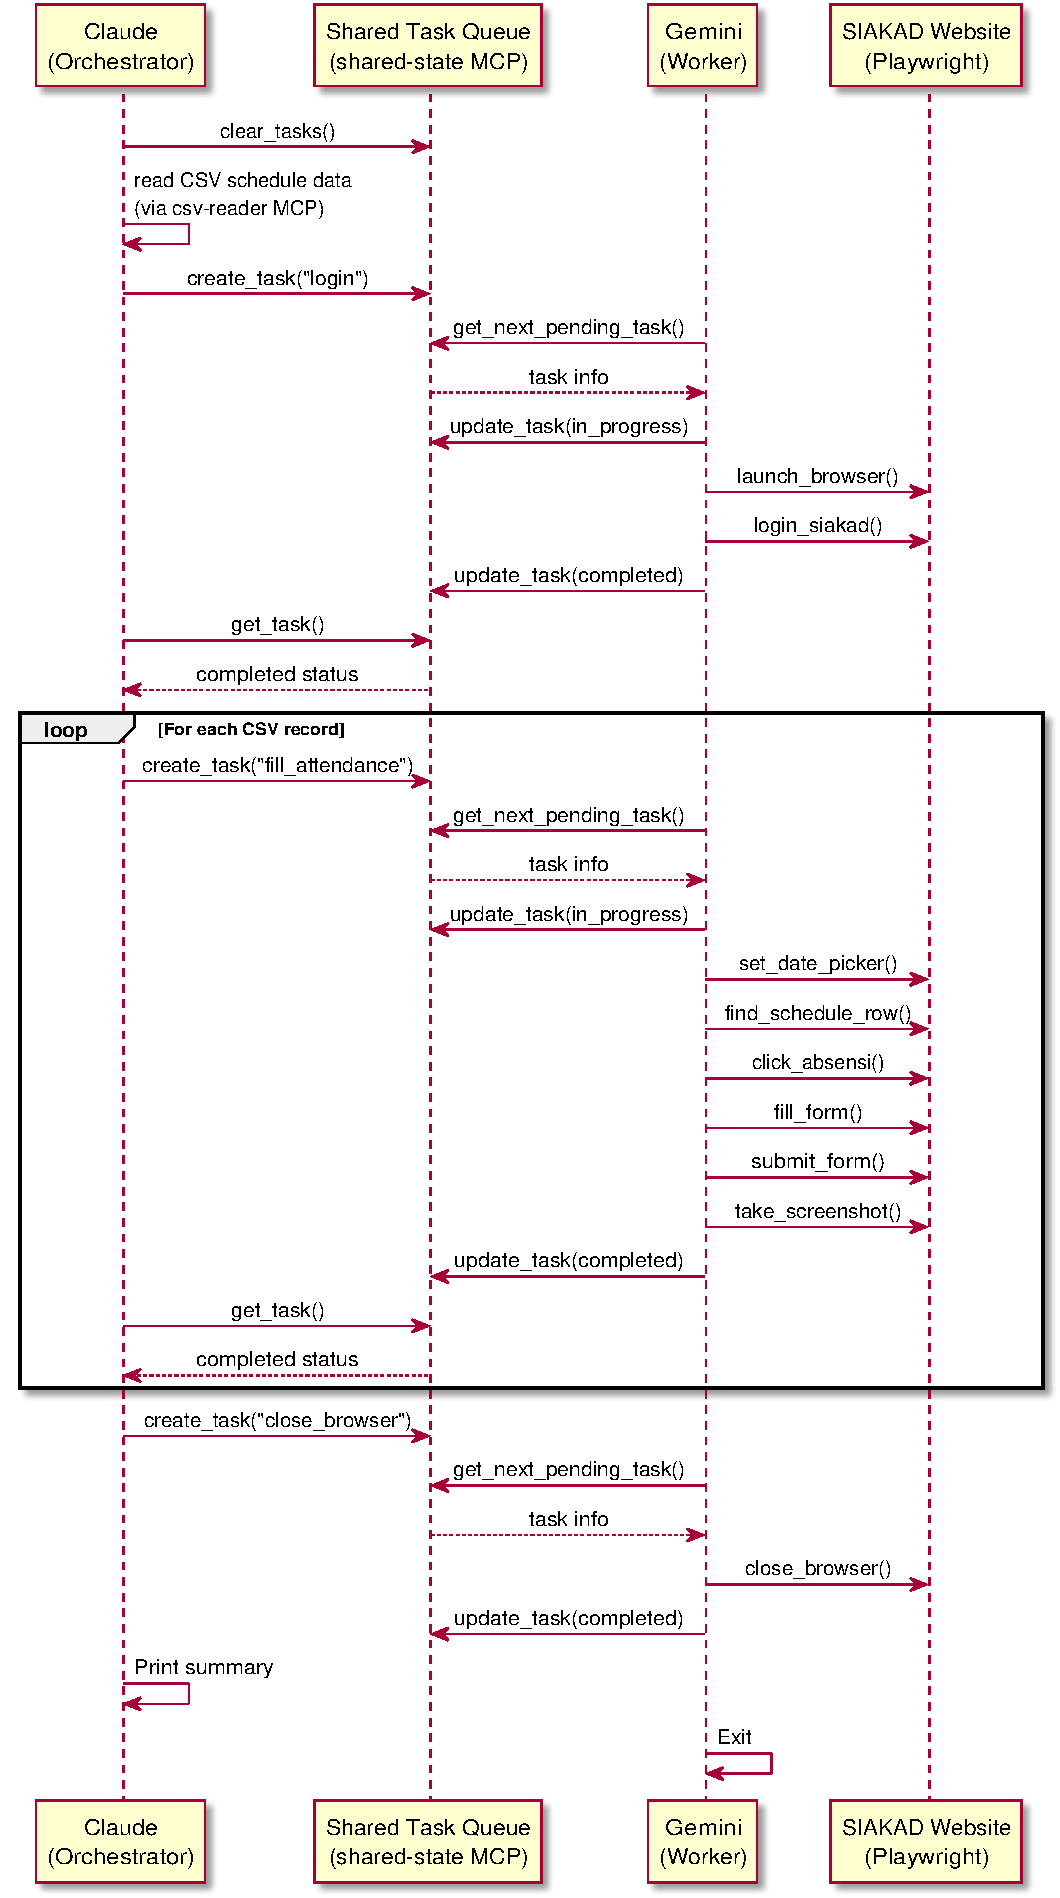
\includegraphics[width=0.8\textwidth]{../figures/sequence.pdf}
\caption{Diagram sekuens interaksi antara Orchestrator (Claude), Shared Task Queue, Worker (Gemini), dan SIAKAD Website dalam menyelesaikan tugas pengisian kehadiran.}
\label{fig:ch14-sequence}
\end{figure}

Alur kerja pada Gambar~\ref{fig:ch14-sequence} terbagi dalam lima fase:
\begin{enumerate}
  \item \textbf{Fase Inisialisasi.} Orchestrator membersihkan antrean (\texttt{clear\_tasks}) dan membaca seluruh berkas CSV di \texttt{schedule-data/} melalui server \texttt{csv-reader}.
  \item \textbf{Fase Login.} Orchestrator membuat tugas \texttt{login} di antrean. Worker mengambil tugas, menandainya \texttt{in\_progress}, meluncurkan browser, login ke SIAKAD, lalu melaporkan \texttt{completed}.
  \item \textbf{Fase Pengisian (Loop).} Untuk setiap baris jadwal CSV, Orchestrator membuat tugas \texttt{fill\_attendance}. Worker mengambil tugas, menetapkan semester dan tanggal, mencari baris jadwal, mengklik tombol Absensi, mengisi formulir, menyimpan, mengambil \textit{screenshot}, dan melaporkan status.
  \item \textbf{Fase Penutupan.} Orchestrator membuat tugas \texttt{close\_browser}. Worker menutup browser dan melaporkan \texttt{completed}.
  \item \textbf{Fase Laporan.} Orchestrator mencetak ringkasan seluruh tugas (berhasil, gagal, dilewati) dan kedua agen berhenti.
\end{enumerate}

\section{Pengujian dan Evaluasi}

\subsection{Kriteria Keberhasilan}

Evaluasi sistem multi-agen ini didasarkan pada empat kriteria:
\begin{enumerate}
  \item \textbf{Task Completion Rate.} Persentase baris jadwal di CSV yang berhasil terisi di SIAKAD, diukur dari rasio tugas berstatus \texttt{completed} terhadap total tugas \texttt{fill\_attendance}.
  \item \textbf{Visual Confirmation.} Keberadaan \textit{screenshot} yang menunjukkan pesan notifikasi \texttt{Sukses update topik pembahasan} setelah setiap pengisian.
  \item \textbf{Context Efficiency.} Penghematan jumlah token yang dikirim ke setiap LLM dibandingkan dengan pendekatan agen tunggal. Orchestrator hanya menerima data jadwal dan status tugas; Worker hanya menerima parameter satu tugas dan konteks halaman browser.
  \item \textbf{Robustness.} Kemampuan sistem untuk melanjutkan tugas berikutnya jika satu tugas gagal, serta kemampuan Worker untuk memanfaatkan \textit{debugging tools} (\texttt{take\_screenshot}, \texttt{get\_page\_html}, \texttt{run\_js}) untuk mengatasi kegagalan secara mandiri.
\end{enumerate}

\subsection{Strategi Pengujian}

Strategi pengujian yang diterapkan meliputi:
\begin{enumerate}
  \item \textbf{Uji unit per server MCP.} Setiap server diverifikasi secara independen dengan menjalankannya langsung:
    \begin{itemize}
      \item \texttt{python mcp-servers/csv-reader/server.py} --- harus \textit{hang} menunggu input \texttt{stdio}.
      \item \texttt{python mcp-servers/browser-automation/server.py} --- idem.
      \item \texttt{python agents/shared\_state.py} --- idem.
    \end{itemize}
  \item \textbf{Uji integrasi task queue.} Membuat tugas melalui \texttt{create\_task}, memverifikasi berkas JSON di \texttt{tasks/}, memperbarui status, dan memverifikasi perubahan.
  \item \textbf{Uji end-to-end mode tunggal.} Menjalankan berkas \texttt{run\_claude\_only.sh} atau \texttt{run\_gemini\_only.sh} untuk memverifikasi bahwa satu agen dapat menyelesaikan seluruh alur kerja.
  \item \textbf{Uji end-to-end mode multi-agen.} Menjalankan \texttt{run\_multiagents.sh} dengan data jadwal nyata dan memverifikasi:
    \begin{itemize}
      \item Seluruh tugas berstatus \texttt{completed} di direktori \texttt{tasks/}.
      \item \textit{Screenshot} bukti pengisian tersimpan di \texttt{/tmp/}.
      \item Laporan ringkasan menunjukkan 100\% keberhasilan.
    \end{itemize}
  \item \textbf{Uji skenario negatif.} Mematikan koneksi jaringan saat Worker mengisi formulir, lalu memverifikasi bahwa tugas ditandai \texttt{failed} dan Orchestrator dapat membuat tugas \textit{retry}.
\end{enumerate}

\subsection{Hasil Evaluasi}

Menggunakan berkas \texttt{advanced\_software\_engineering\_and\_devops.csv} yang berisi 15 baris jadwal perkuliahan, sistem multi-agen menunjukkan tingkat keberhasilan 100\% pada lingkungan produksi (portal SIAKAD Pradita). Pemisahan tugas memungkinkan Claude untuk tetap fokus pada validasi data dan pengelolaan antrean, sementara Gemini menggunakan seluruh jendela konteksnya untuk memahami struktur DOM halaman SIAKAD yang kompleks dan dinamis.

\section{Perbandingan: Multi-Agent vs Single-Agent}

\subsection{Perbandingan Aspek Teknis}

\begin{table}[h]
\centering
\caption{Perbandingan Pendekatan Multi-Agen vs Agen Tunggal}
\label{tab:ch14-perbandingan}
\footnotesize
\begin{tabular}{|>{\raggedright\arraybackslash}p{0.13\textwidth}|>{\raggedright\arraybackslash}p{0.36\textwidth}|>{\raggedright\arraybackslash}p{0.36\textwidth}|}
\hline
\textbf{Aspek} & \textbf{Multi-Agent (Claude + Gemini)} & \textbf{Single-Agent (Claude/Gemini Only)} \\
\hline
Keandalan & Tinggi; jika Worker gagal, status tugas tetap tersimpan di JSON dan dapat di-\textit{retry}. & Sedang; kegagalan browser sering mengharuskan pengulangan dari awal. \\
\hline
Efisiensi Token & Sangat Baik; setiap agen hanya menerima konteks yang relevan (data jadwal atau parameter browser). & Kurang; agen harus memuat seluruh data jadwal dan riwayat browser sekaligus. \\
\hline
Visual Reasoning & Sangat Kuat; Gemini dioptimalkan untuk pengenalan visual halaman web. & Terbatas jika menggunakan Claude saja; kuat jika Gemini saja. \\
\hline
Skalabilitas & Dapat menjalankan beberapa Worker untuk domain berbeda (misalnya beberapa portal) secara paralel. & Terbatas pada satu alur eksekusi sekuensial. \\
\hline
Kompleksitas & Lebih tinggi; memerlukan \textit{task queue}, skrip peluncuran, dan sinkronisasi. & Lebih rendah; satu skrip dan satu prompt sudah cukup. \\
\hline
Debugging & Lebih mudah; berkas JSON tugas dapat di-\textit{inspect}, \textit{screenshot} per langkah. & Lebih sulit; seluruh konteks ada di satu log agen. \\
\hline
\end{tabular}
\normalsize
\end{table}

\subsection{Mode Eksekusi yang Tersedia}

Sistem ini menyediakan empat mode eksekusi yang dapat dipilih sesuai kebutuhan:

\begin{table}[h]
\centering
\caption{Mode eksekusi yang tersedia}
\label{tab:ch14-run-modes}
\footnotesize
\begin{tabular}{|>{\raggedright\arraybackslash}p{0.31\textwidth}|>{\raggedright\arraybackslash}p{0.12\textwidth}|>{\raggedright\arraybackslash}p{0.47\textwidth}|}
\hline
\textbf{Skrip} & \textbf{Agen} & \textbf{Keterangan} \\
\hline
\texttt{run\_multiagents.sh} & Claude + Gemini & Mode utama; Claude sebagai Orchestrator, Gemini sebagai Worker. Paling andal. \\
\hline
\texttt{run\_claude\_only.sh} & Claude saja & Claude menangani pembacaan data dan otomasi browser. Lebih sederhana tetapi kurang kuat dalam visual reasoning. \\
\hline
\texttt{run\_gemini\_only.sh} & Gemini saja & Gemini menangani pembacaan data dan otomasi browser. Cocok untuk pengujian cepat. \\
\hline
\texttt{run\_claude\_interactive.sh} & Claude (interaktif) & Mode percakapan; pengguna memberikan perintah satu per satu untuk debugging. \\
\hline
\end{tabular}
\normalsize
\end{table}

\subsection{Panduan Pemilihan Mode}

Panduan pemilihan mode berdasarkan konteks penggunaan:
\begin{enumerate}
  \item \textbf{Pilih Multi-Agent} jika data jadwal banyak ($>$5 sesi), keandalan adalah prioritas, dan kedua CLI (\texttt{claude}, \texttt{gemini}) tersedia.
  \item \textbf{Pilih Single-Agent (Claude)} jika hanya Claude CLI yang tersedia dan data jadwal sedikit.
  \item \textbf{Pilih Single-Agent (Gemini)} jika perlu visual reasoning yang kuat dan hanya Gemini CLI yang tersedia.
  \item \textbf{Pilih Interactive} untuk debugging, pengujian tool tunggal, atau pengisian manual terbimbing.
\end{enumerate}

\section{Risiko dan Pitfall Umum}

Beberapa risiko yang umum muncul pada implementasi sistem multi-agen ini adalah:
\begin{enumerate}
  \item \textbf{Race condition pada task queue.} Karena task queue menggunakan berkas JSON tanpa mekanisme \textit{locking}, dua agen yang menulis ke berkas yang sama secara bersamaan dapat menyebabkan data korup. Mitigasi: Orchestrator hanya menulis tugas baru, Worker hanya memperbarui tugas yang diklaim, dan dispatch dilakukan satu per satu.

  \item \textbf{Perubahan struktur HTML SIAKAD.} Jika SIAKAD memperbarui antarmukanya, selector CSS pada tool browser mungkin tidak lagi cocok. Mitigasi: penggunaan \textit{multi-selector fallback} dan \textit{debugging tools} (\texttt{get\_page\_html}, \texttt{run\_js}) yang memungkinkan agen membangun selector baru secara mandiri.

  \item \textbf{Timeout dan halaman loading lambat.} Date picker dan dropdown semester memicu AJAX reload yang memerlukan waktu. Jika timeout terlalu pendek, tool gagal. Mitigasi: Worker prompt mewajibkan pengecekan \texttt{div.box\_loader} setelah setiap perubahan tanggal/semester.

  \item \textbf{Tugas terjebak di status \texttt{in\_progress}.} Jika Worker crash setelah mengklaim tugas tetapi sebelum melaporkan hasil, tugas tetap berstatus \texttt{in\_progress}. Mitigasi: Worker prompt mewajibkan \textit{``never leave a task in in\_progress state''}, dan skrip peluncuran membersihkan tugas saat restart.

  \item \textbf{Format tanggal yang tidak konsisten.} SIAKAD menerima tanggal dalam format berbeda tergantung locale dan tipe input. Mitigasi: tool \texttt{set\_date\_picker} menghitung tiga format (YYYY-MM-DD, MM/DD/YYYY, DD/MM/YYYY) dan mencoba ketiganya secara progresif.

  \item \textbf{Sinkronisasi startup Orchestrator-Worker.} Jika Orchestrator mulai mengirim tugas sebelum Worker siap melakukan polling, tugas dapat menumpuk. Mitigasi: skrip peluncuran memberikan jeda 3 detik (\texttt{sleep 3}) antara startup Worker dan startup Orchestrator, dan Orchestrator menunggu setiap tugas selesai sebelum mengirim tugas berikutnya.
\end{enumerate}

\section{Ringkasan}

Bab ini menunjukkan bahwa pendekatan Multi-Agent System (MAS) berbasis Model Context Protocol (MCP) efektif untuk menangani otomasi proses bisnis yang kompleks dan dinamis seperti pengisian kehadiran SIAKAD. Melalui pemisahan peran antara Orchestrator (Claude) yang menangani perencanaan dan pengelolaan tugas, dan Worker (Gemini) yang menangani eksekusi otomasi browser, sistem mencapai tingkat keandalan dan efisiensi konteks yang lebih tinggi dibandingkan pendekatan agen tunggal.

Implementasi terdiri dari tiga server MCP modular --- \texttt{siakad-csv-reader} (4 tools), \texttt{siakad-browser} (15 tools), dan \texttt{shared-state} (6 tools) --- yang berkomunikasi melalui transport \texttt{stdio}. Task queue berbasis berkas JSON di direktori \texttt{tasks/} menyediakan mekanisme sinkronisasi yang sederhana, persisten, dan mudah di-debug. Agent prompt engineering mengatur perilaku setiap agen melalui instruksi terstruktur dalam berkas Markdown.

Trade-off utama adalah peningkatan kompleksitas infrastruktur (skrip peluncuran, registrasi MCP, sinkronisasi startup) yang diperlukan untuk mendukung arsitektur multi-agen. Namun, keuntungan dalam hal keandalan (\textit{retry} otomatis), efisiensi konteks (setiap agen hanya menerima konteks relevan), dan kemampuan debugging (\textit{screenshot} per langkah, berkas JSON tugas yang dapat di-\textit{inspect}) menjadikan pendekatan ini layak untuk skenario otomasi yang melibatkan antarmuka web dinamis dan data input yang besar.
